% =====================================================================
\chapter{Modelagem do software}\label{cap:modelagem}
% =====================================================================

A modelagem usou a UML para casos de uso e classes \parencite{booch2006} e um diagrama entidade-relacionamento para o banco. Os atores são o \textbf{dispositivo} (datalogger que envia os lotes), o \textbf{visualizador} (consulta e exporta), o \textbf{operador} (também reconhece eventos e ajusta alarmes), o \textbf{administrador} (também gerencia usuários, auditoria, backups e parâmetros) e o \textbf{agendador} do servidor. A \autoref{fig:casos-uso} mostra os casos de uso; a herança entre atores representa os perfis cumulativos, e os «include» mostram que todo lote é validado e toda alteração é auditada.

\begin{figure}[htb]
  \caption{Diagrama de casos de uso}\label{fig:casos-uso}
  \centering
  \resizebox{0.74\textwidth}{!}{% Diagrama de casos de uso (UML)
\begin{tikzpicture}[
  font=\scriptsize,
  uc/.style={ellipse, draw=azul, fill=azulclaro, line width=0.6pt, minimum width=3.7cm, minimum height=0.8cm, align=center, inner sep=1pt},
  inc/.style={ellipse, draw=azul, dashed, fill=white, line width=0.6pt, minimum width=3.0cm, minimum height=0.72cm, align=center, inner sep=1pt},
  assoc/.style={line width=0.5pt, color=tinta},
  heranca/.style={-{Triangle[open, length=2.4mm, width=2.4mm]}, line width=0.5pt, color=tinta},
  inclui/.style={-{Stealth[length=1.8mm]}, dashed, line width=0.5pt, color=cinza},
]
\newcommand{\ator}[3]{%
  \begin{scope}[shift={#2}, line width=0.6pt, color=tinta]
    \draw (0,0.42) circle (0.13);
    \draw (0,0.29) -- (0,-0.08);
    \draw (-0.22,0.16) -- (0.22,0.16);
    \draw (0,-0.08) -- (-0.18,-0.38);
    \draw (0,-0.08) -- (0.18,-0.38);
    \node[font=\scriptsize\bfseries, align=center, below] at (0,-0.4) {#3};
    \coordinate (#1) at (0.25,0.1);
    \coordinate (#1-topo) at (0,0.6);
    \coordinate (#1-base) at (0,-0.95);
  \end{scope}}

\draw[rounded corners=6pt, draw=azul, line width=0.8pt] (-2.3,-5.15) rectangle (5.6,4.3);
\node[font=\scriptsize\bfseries, color=azul] at (1.65,4.02) {Sistema de monitoramento (banco + servidor + painel)};

\node[uc] (u1) at (0,3.3) {UC01 Enviar lote\\de leituras};
\node[uc] (u2) at (0,2.3) {UC02 Acompanhar painel\\em tempo real};
\node[uc] (u3) at (0,1.3) {UC03 Consultar gráficos,\\histórico e exportar};
\node[uc] (u4) at (0,0.3) {UC04 Reconhecer\\eventos};
\node[uc] (u5) at (0,-0.7) {UC05 Ajustar regras\\de alarme e sensores};
\node[uc] (u6) at (0,-1.7) {UC06 Gerenciar\\usuários};
\node[uc] (u7) at (0,-2.7) {UC07 Auditar e verificar\\integridade};
\node[uc] (u8) at (0,-3.7) {UC08 Fazer e verificar\\backup};
\node[uc] (u9) at (0,-4.6) {UC09 Arquivar dados\\e criar partições};

\node[inc] (i1) at (3.85,3.55) {Validar leituras\\e datas};
\node[inc] (i2) at (3.85,2.55) {Gerar eventos\\e alarmes};
\node[inc] (i3) at (3.85,-0.7) {Registrar na\\auditoria};

\ator{disp}{(-4.3,3.2)}{Dispositivo\\(datalogger)}
\ator{vis}{(-4.3,1.55)}{Visualizador}
\ator{ope}{(-4.3,-0.45)}{Operador}
\ator{adm}{(-4.3,-2.5)}{Administrador}
\ator{age}{(-4.3,-4.35)}{Agendador\\(servidor)}

\draw[assoc] (disp) -- (u1.west);
\draw[assoc] (vis) -- (u2.west);
\draw[assoc] (vis) -- (u3.west);
\draw[assoc] (ope) -- (u4.west);
\draw[assoc] (ope) -- (u5.west);
\draw[assoc] (adm) -- (u6.west);
\draw[assoc] (adm) -- (u7.west);
\draw[assoc] (adm) -- (u8.west);
\draw[assoc] (age) -- (u8.west);
\draw[assoc] (age) -- (u9.west);

\draw[heranca] (ope-topo) -- (vis-base);
\draw[heranca] (adm-topo) -- (ope-base);

\draw[inclui] (u1.east) -- node[above, font=\tiny, sloped]{«include»} (i1.west);
\draw[inclui] (u1.east) -- node[below, font=\tiny, sloped]{«include»} (i2.west);
\draw[inclui] (u4.east) -- node[above, font=\tiny, sloped]{«include»} (i3.west);
\draw[inclui] (u5.east) -- node[above, font=\tiny]{«include»} (i3.west);
\draw[inclui] (u6.east) -- node[below, font=\tiny, sloped]{«include»} (i3.west);
\end{tikzpicture}
}
  \fonte{Elaborado pelos autores (2026).}
\end{figure}

\newcommand{\linhauc}[2]{\textbf{#1} & #2 \\ \hline}

\begin{quadro}[htb]
  \caption{Caso de uso UC01 -- Enviar lote de leituras}\label{qua:uc01}
  \footnotesize
  \begin{tabularx}{\textwidth}{|L{2.8cm}|Y|}
    \hline
    \linhauc{Ator / pré-condição}{Dispositivo; estação ativa com chave de API cadastrada.}
    \textbf{Fluxo básico} & 1. O dispositivo envia o lote para \texttt{/api/ingest} com a chave no cabeçalho. 2. O banco identifica a estação pelo hash da chave e registra falha de transmissão se o lote atrasou. 3. Classifica cada leitura e separa as rejeitadas. 4. Grava as válidas e novas; os \textit{triggers} descartam valores fora da faixa, calculam a chuva acumulada e geram alarmes. 5. Registra a transmissão e avisa os painéis em tempo real. \\ \hline
    \textbf{Alternativos e exceções} & Leituras repetidas são ignoradas sem gerar eventos. Leituras inválidas geram um evento \texttt{LEITURA\_REJEITADA} por motivo, e o resto do lote é gravado. Chave inválida: envio recusado e auditado. Banco fora do ar: o lote vai para a fila de contingência. \\ \hline
    \linhauc{Regra}{A data de recebimento é sempre o relógio do servidor.}
  \end{tabularx}
  \fonte{Elaborado pelos autores (2026).}
\end{quadro}

\begin{quadro}[htb]
  \caption{Caso de uso UC07 -- Auditar e verificar integridade}\label{qua:uc07}
  \footnotesize
  \begin{tabularx}{\textwidth}{|L{2.8cm}|Y|}
    \hline
    \linhauc{Ator / pré-condição}{Administrador autenticado.}
    \textbf{Fluxo básico} & 1. O administrador abre a auditoria; a verificação roda sozinha. 2. O banco percorre a trilha em ordem, recalcula o SHA-256 de cada registro com o hash do anterior e compara com o gravado. 3. O administrador filtra por ação, objeto, usuário e período e abre o antes e depois de cada alteração. \\ \hline
    \linhauc{Alternativo}{Registro alterado ou removido: a tela mostra o número do primeiro registro com problema.}
    \linhauc{Regra}{A trilha é somente de inclusão; desligar essa proteção é um comando de estrutura e também é auditado.}
  \end{tabularx}
  \fonte{Elaborado pelos autores (2026).}
\end{quadro}

O diagrama de classes (\autoref{fig:classes}) representa o domínio. Suas operações estão no próprio banco, como funções e \textit{triggers} em PL/pgSQL: \texttt{receberLote} é \texttt{fn\_receber\_lote}, \texttt{reconhecer} é \texttt{fn\_reconhecer\_eventos} e \texttt{verificarIntegridade} é \texttt{fn\_verificar\_auditoria}.

\begin{figure}[htb]
  \caption{Diagrama de classes do domínio}\label{fig:classes}
  \centering
  \resizebox{0.84\textwidth}{!}{% Diagrama de classes do domínio (pgf-umlcd)
\begin{tikzpicture}[font=\scriptsize]
\begin{class}[text width=3.3cm]{Cliente}{0,0}
  \attribute{nome : texto}
  \attribute{cidade : texto}
  \attribute{uf : texto}
\end{class}

\begin{class}[text width=4.3cm]{Dispositivo}{5.2,0}
  \attribute{nome : texto}
  \attribute{status : Status}
  \attribute{ultimaComunicacao : data/hora}
  \attribute{intervaloTransmissao : int}
  \operation{+ receberLote(leituras) : int}
  \operation{+ verificarComunicacao()}
\end{class}

\begin{class}[text width=3.6cm]{Usuario}{0,-4.0}
  \attribute{login : texto}
  \attribute{senhaHash : bcrypt}
  \attribute{perfil : Perfil}
  \attribute{bloqueadoAte : data/hora}
  \operation{+ login(senha) : Sessao}
  \operation{+ alterarSenha(atual, nova)}
\end{class}

\begin{class}[text width=3.5cm]{Sessao}{0,-8.1}
  \attribute{tokenHash : SHA-256}
  \attribute{expiraEm : data/hora}
  \operation{+ validar() : Usuario}
\end{class}

\begin{class}[text width=3.6cm]{Sensor}{10.6,1.0}
  \attribute{parametro : texto}
  \attribute{limiteMin, limiteMax : num}
  \operation{+ valida(valor) : bool}
\end{class}

\begin{class}[text width=3.6cm]{RegraAlarme}{10.6,-2.3}
  \attribute{parametro : texto}
  \attribute{condicao : ACIMA/ABAIXO}
  \attribute{limite : num}
  \attribute{nivel : Nivel}
  \operation{+ violada(valor) : bool}
\end{class}

\begin{class}[text width=3.9cm]{Leitura}{5.2,-4.0}
  \attribute{dataHora : data/hora}
  \attribute{temperatura, umidade : num}
  \attribute{chuva, chuvaAcumulada : num}
  \attribute{vento, direcao, radiacao : num}
  \attribute{recebidoEm : data/hora}
\end{class}

\begin{class}[text width=3.6cm]{Evento}{5.2,-8.0}
  \attribute{dataHora : data/hora}
  \attribute{tipo : TipoEvento}
  \attribute{mensagem : texto}
  \attribute{reconhecidoEm : data/hora}
  \operation{+ reconhecer()}
\end{class}

\begin{class}[text width=4.4cm]{Auditoria}{10.6,-7.0}
  \attribute{dataHora, login, ip}
  \attribute{acao, antes, depois}
  \attribute{hashAnterior, hash}
  \operation{+ verificarIntegridade() : bool}
\end{class}

\association{Cliente}{}{1}{Dispositivo}{}{0..*}
\association{Cliente}{}{0..1}{Usuario}{}{0..*}
\composition{Usuario}{}{1}{Sessao}{0..*}
\composition{Dispositivo}{}{1}{Sensor}{1..*}
\composition{Dispositivo}{}{1}{RegraAlarme}{0..*}
\composition{Dispositivo}{}{1}{Leitura}{0..*}
\association{RegraAlarme}{gera}{0..1}{Evento}{}{0..*}
\association{Leitura}{origina}{1}{Evento}{}{0..*}
\association{Usuario}{reconhece}{0..1}{Evento}{}{0..*}
\end{tikzpicture}
}
  \fonte{Elaborado pelos autores (2026).}
\end{figure}

\section{Modelo de dados}

O modelo físico tem 14 tabelas (\autoref{fig:der}), num diagrama gerado do catálogo do banco para corresponder exatamente ao implementado. A tabela \texttt{leitura} tem uma linha por estação por minuto, chave primária (\texttt{id\_dispositivo}, \texttt{data\_hora}) e partições mensais; os meses antigos são movidos inteiros para \texttt{leitura\_arquivo}, com índice BRIN, e resumidos em \texttt{leitura\_diaria}. Os eventos ficam numa tabela única, no formato de log, com cinco tipos: transmissão OK, falha de transmissão, falha de sensor, alarme e leitura rejeitada. As regras de alarme cadastradas são chuva acumulada acima de 50~mm (crítico), vento acima de 17~m/s, temperatura acima de 35~°C e umidade abaixo de 20\,\% (alerta).

\begin{figure}[p]
  \caption{Modelo de dados (diagrama entidade-relacionamento)}\label{fig:der}
  \centering
  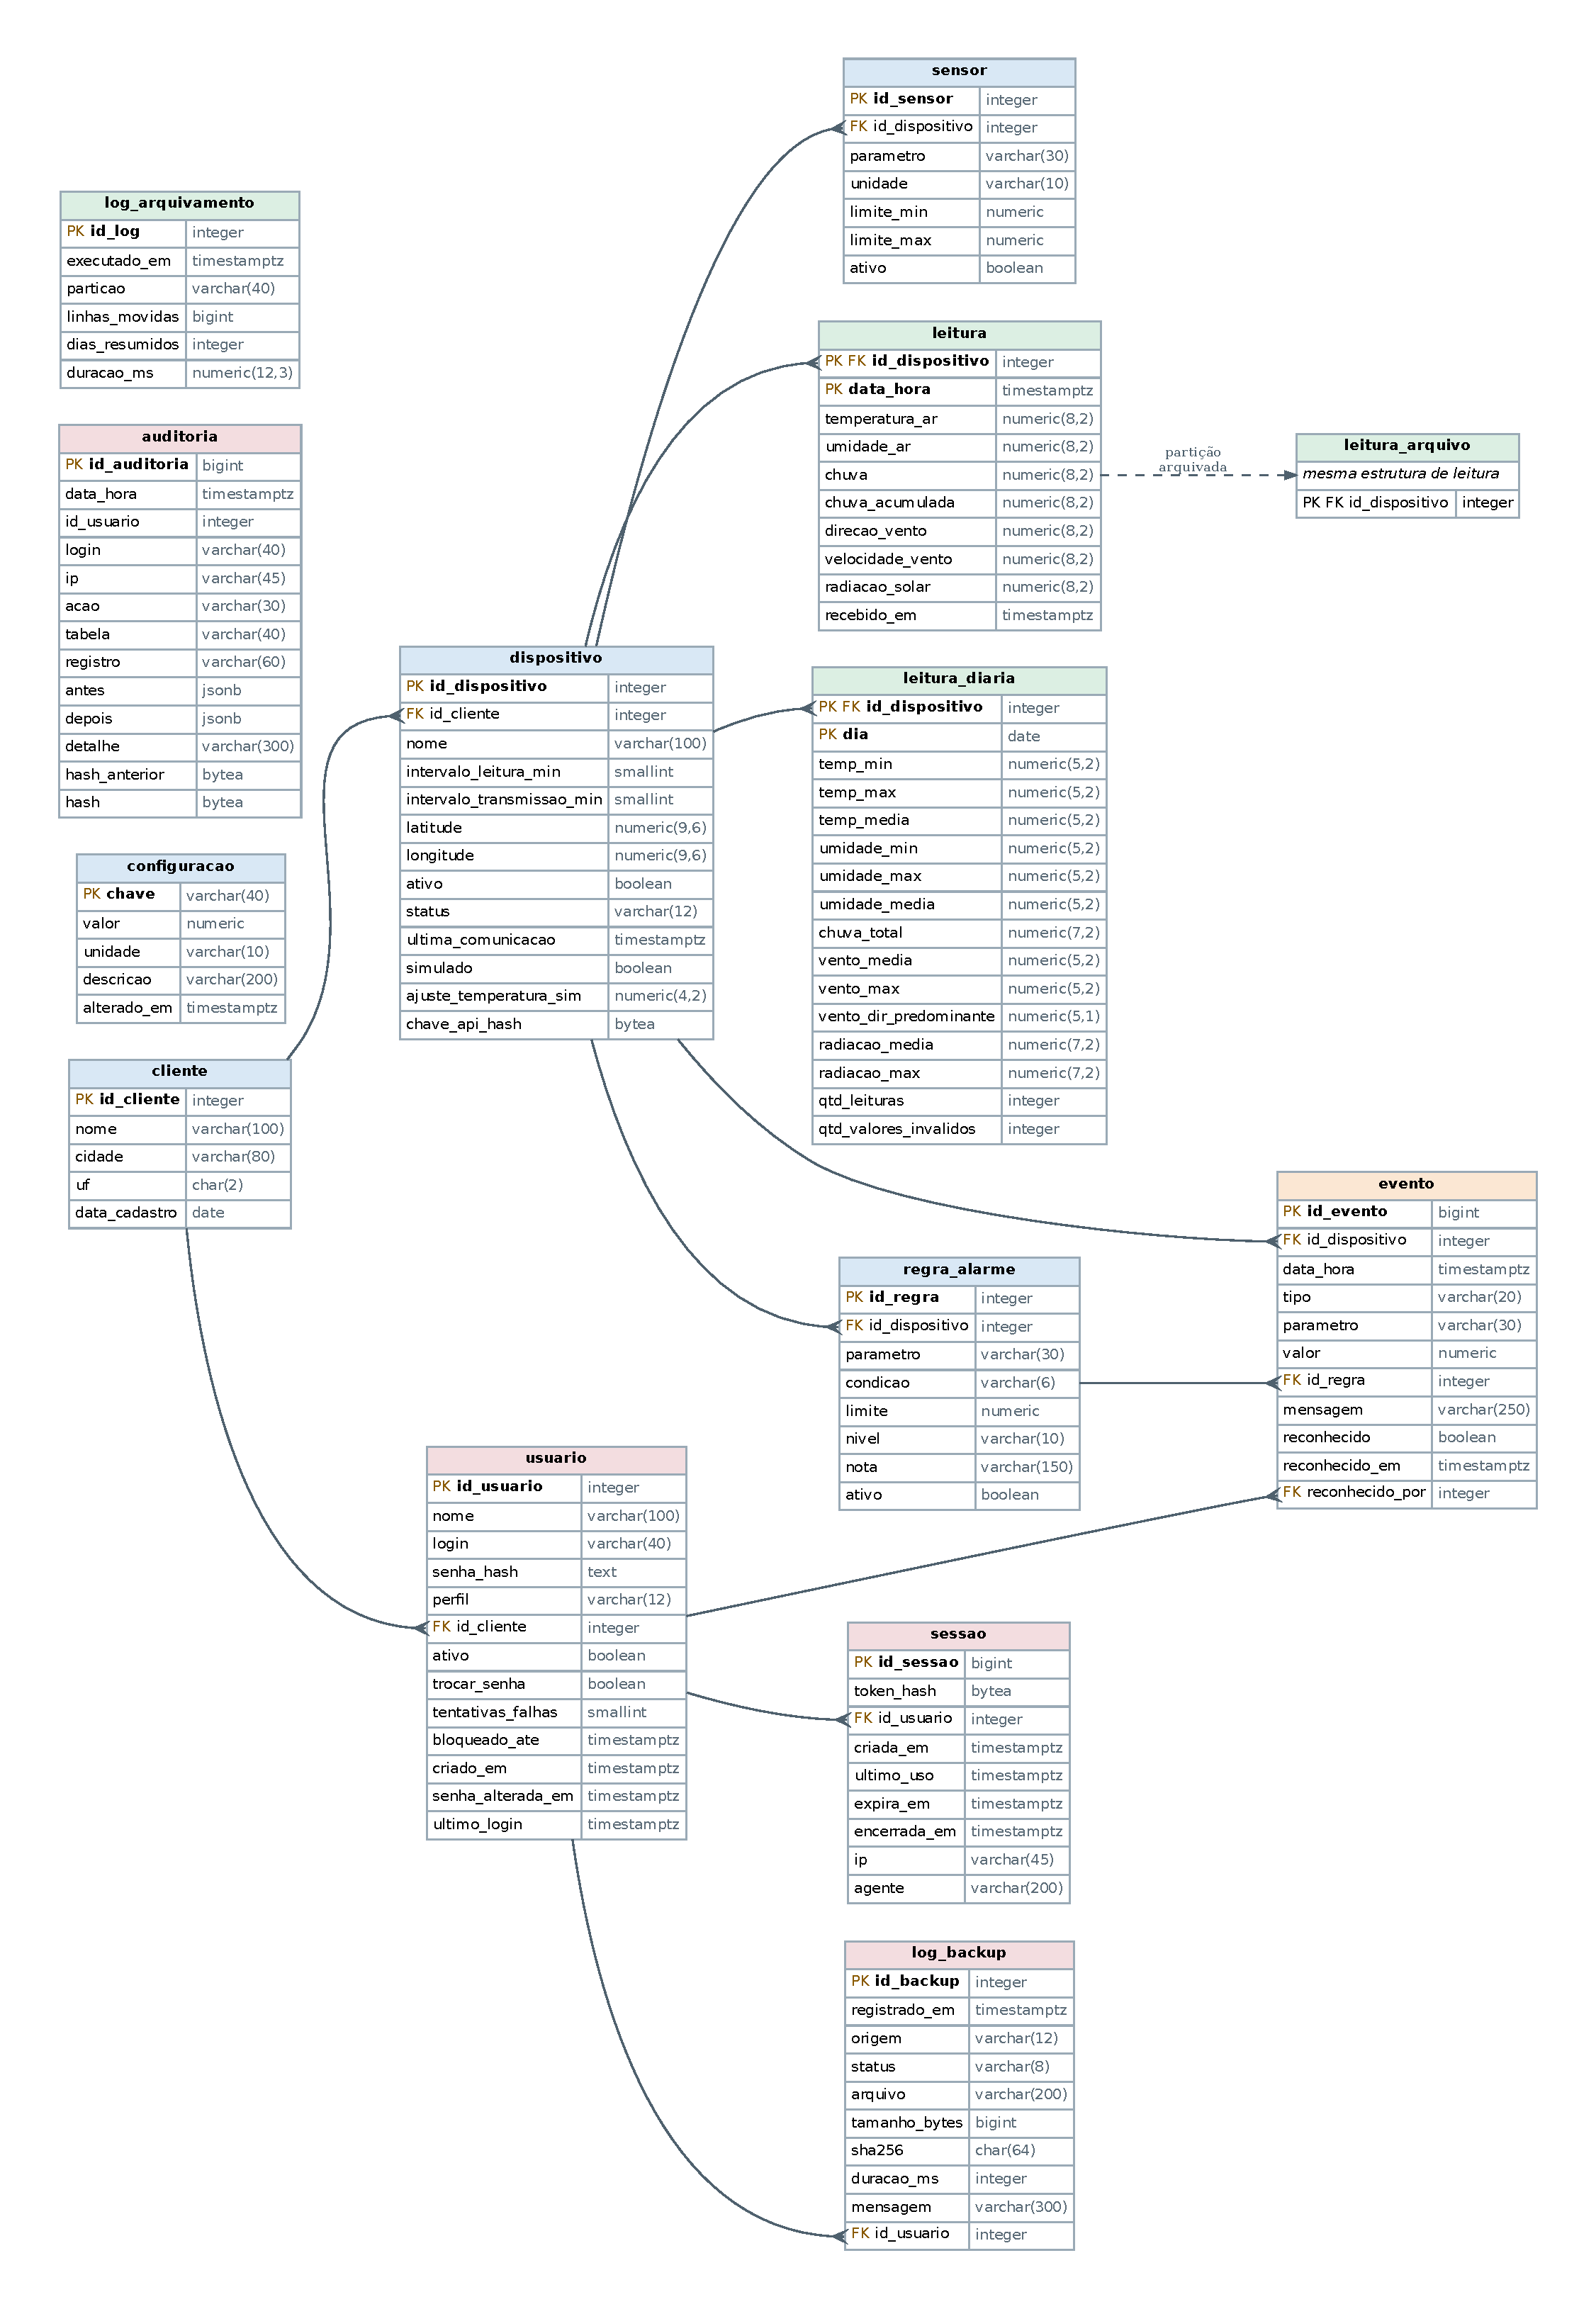
\includegraphics[height=0.84\textheight,width=\textwidth,keepaspectratio]{figuras/der.pdf}
  \fonte{Elaborado pelos autores (2026), gerado do catálogo do PostgreSQL com Graphviz.}
\end{figure}

\section{Regras implementadas no banco}

Todo dado entra por \texttt{fn\_receber\_lote}, que não tem parâmetro de data: o recebimento é sempre \texttt{now()}. Numa única instrução SQL, a função lê o JSON (valores mal formatados viram nulo, sem abortar o lote), classifica cada leitura (data no futuro além de 2~min, mais antiga que 7 dias ou de mês sem partição ativa são rejeitadas), grava um evento por motivo de rejeição e insere só as leituras válidas e novas, o que corrigiu as falhas de sensor ``fantasmas'' da primeira versão. Como defesa adicional, o \textit{trigger} da tabela recusa data no futuro mesmo em inclusões diretas.

Na auditoria, um \textit{trigger} define a data com o relógio do servidor, identifica o usuário pela sessão e calcula o SHA-256 do registro concatenado ao hash do anterior, sob um bloqueio que garante a ordem da corrente. Diariamente, o banco arquiva os meses antigos (\texttt{DETACH} e \texttt{ATTACH PARTITION}) e cria as partições dos dois meses seguintes.
